\chapter{BLAST}

\section{背景}
对于研究序列同源性,序列的相似程度问题,序列比对算法是非常重要的工具。双序列比对可以采用基于动态规划算法的Needleman-Wunsch和Smith-Waterman算法,虽然精度高,但是计算消耗大,因此当与数据库进行比对时,这两种算法就显得力不从心。Blast采用启发式算法,通过丢失灵敏度来减少运行时间,以实现序列与大规模数据库的比对。


\section{BLAST}
BLAST(Basic Local Alignment Search Tool)算法的基本思想是通过产生数量更少的但质量更好的增强点来提高比对的速度。算法的原理主要分为以下五步:(1)过滤:首先过滤掉低复杂度区域,即含有大量重复的序列;(2)Seeding:将Query序列中每k个字组合成一个表,即将一个序列拆分成多个连续的‘seed words’(通常蛋白质k=3,核酸k=11);(3)比对:列出我们所关心的所有可能的字组,再配合置换矩阵给出高分值的字组并组织成快速搜索树结构或者哈希索引,因此此步骤可以快速搜索出大数据集中的所有匹配序列,找到每个seed words在参考序列中的位置;(4)延伸:当找到seed words的位置后,接下来需要将seed word延伸成长片段,延伸过程中,得分值也在变化,当得分值小于阈值时即停止延伸,最后得到的片段成为高分片段对,HSP(High-scoring segment pair);(5)显著性分析,最后我们使用如下公式计算E值,E值衡量了在随机情况下,数据库存在的比当前匹配分数更好的比对的数目,因此可以用该值作为指标评价HSP比对序列的可信度\par
$$ E = kmne^{-\lambda S}$$
其中,m是数据库长度,n是query的长度,S是HSP分数,其他两个参数是修正系数。
\subsection{BLAST的基本想法}
\begin{enumerate}
    \item 首先将输入序列切分成若干小段——seed words, 对于一个给定的字长 w (usually 3 for proteins and 11 for nucleotides), 将输入序列分成许多连续的 seed words
    \item 通过事先建立的索引表,在数据库中快速定位候选序列,以及在候选序列中的具体位置(通过正确设计索引结果,这一步可以在线性甚至常数时间范围内完成, 从而提高效率)
    \item 通过对所有的seed重复上述操作,就可以得到查询序列与候选序列之间的hit map ——最优比对对应的路径,应当平行于主对角线。
    \item 进一步去掉零散的hits,仅保留沿对角线方向上,有两个及以上连续hits的hit clusters, 以便进一步缩小搜索空间
    \item 以hit cluster为基础,向左右两个方向,延伸扩展,知道总分数的下降超过一个给定的x值之后,停止延伸
    \item 在扩展后的区域,应用动态规划算法,确定最终的比对
\end{enumerate}
\subsection{Word size和积分矩阵}
Word size和积分矩阵是BLAST算法中的两个重要参数。Word size(W)指的是在查询序列中用于匹配数据库序列的单词长度。积分矩阵(scoring matrix)用于计算序列比对的得分。
调整这些参数可以优化BLAST搜索。例如,如果T与W成比例缩放,则较小的word size会增加灵敏度并降低速度。W,T和积分矩阵之间的相互作用至关重要,明智地选择它们是控制BLAST速度和灵敏度最有效的方法

\section{BLAST比对工具}
BLASTP是蛋白序列到蛋白库中的一种查询。库中存在的每条已知序列将逐一地同每条所查序列作一对一的序列比对。\par
BLASTX是核酸序列到蛋白库中的一种查询。先将核酸序列翻译成蛋白序列(一条核酸序列会被翻译成可能的六条蛋白),再对每一条作一对一的蛋白序列比对。\par
BLASTN是核酸序列到核酸库中的一种查询。库中存在的每条已知序列都将同所查序列作一对一地核酸序列比对。\par
TBLASTN是蛋白序列到核酸库中的一种查询。与BLASTX相反,它是将库中的核酸序列翻译成蛋白序列,再同所查序列作蛋白与蛋白的比对。\par
TBLASTX是核酸序列到核酸库中的一种查询。此种查询将库中的核酸序列和所查的核酸序列都翻译成蛋白(每条核酸序列会产生6条可能的蛋白序列),这样每次比对会产生36种比对阵列。

\begin{figure}[ht]
    \centering
    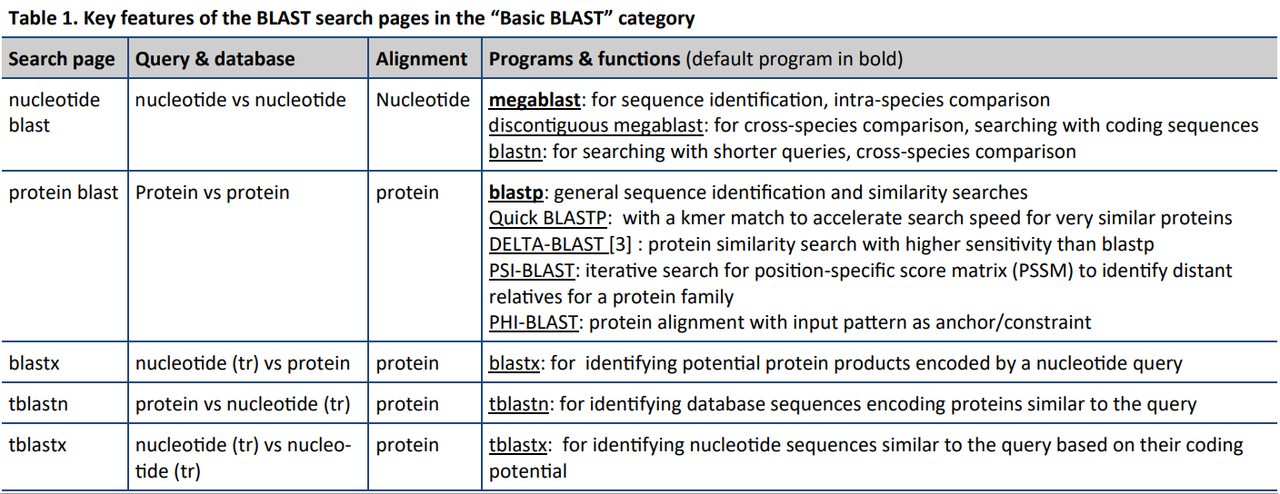
\includegraphics[width=10cm]{figure/blast.PNG}
\end{figure}

其中blastp中又有一些细分的方法,适用于比对不同相似程度的序列。quickblastp适用于快速比较非常相似的蛋白序列;delta-blast相比普通的blastp具有更高的灵敏度;PSI-blast使用PSSM打分矩阵,可以比较蛋白家族中关系较远的序列;PHI-blast将输入模式作为约束的蛋白比对,找到与查询序列具有一样的表达模式且具有同源性的蛋白序列。\par
其中blastn中也有一些细分的方法,具有不同的特点。除去标准方法blastn,magablast使用模糊搜索加快比对速度,用于优化非常相似的序列比较,或鉴定某段核酸序列是否在数据库中;DiscontiguousMagablast比blastn灵敏度更高,用于精确比对,适用于跨物种间的同源比对。\par
此外还有一些特殊功能的blast:
\begin{enumerate}
    \item Primer-BLAST: 使用primer3算法设计引物,并使用BLAST比对所选序列的模板特异性
    \item SmartBlast:可对使用者的蛋白查询进行处理,从数据库中选出5个最佳的蛋白匹配项,并给出一个简明的摘要
    \item lgBLAST:争对种系数据库搜索免疫球蛋白或T细胞受体序列以注释输入的免疫球蛋白序列,可以报告D/J区的相似对象;注释数据中的不同结构域
    \item MOLE-BLAST:从选定目标数据库中识别输入核苷酸序列的相邻序列(使用blast),然后使用多重序列比对(MUSCLE)根据序列相似性聚类。
    \item VecScreen:根据已知载体库和其他人工序列筛选输入的核酸序列,确定污染
    \item CD-search:与保守结构域数据库做比较,根据数据库检索蛋白序列进行功能分析
    \item CDART:识别输入蛋白序列中的保守结构域,然后寻找含有这些保守结构域额其他序列。
    \item Targeted loci:从细菌和古菌中的16S rRNA,或真菌的18S,28S和ITS中搜索仔细挑选的核苷酸序列,用于物种鉴定的需要
\end{enumerate}

\section{blast本地化安装配置}
配置local BLAST可以有效增加BLAST稳定性和比对速度。local BLAST由ncbi BLAST和数据库组成,用户可根据自己需要的数据库选择性下载,如rna\_reference数据库300GB左右,rna\_select数据库不超过50GB。

\subsection{准备工作}
源码安装BLAST
\begin{lstlisting}
# 复制安装包到目标目录
cp /rd1/home/public/BLAST/BLAST_TOOL/ncbi-blast-2.13.0+-x64-linux.tar.gz ~/install 

# 解压解包
gunzip ncbi-blast-2.13.0+-x64-linux.tar.gz
tar xvf ncbi-blast-2.13.0+-x64-linux.tar

# 复制可执行程序
cp -rf install/ncbi-blast-2.13.0+/bin/ ~/bin/blast_bin/

# 用户根目录隐藏文件.ncbirc用于指定数据库文件位置
# Specifies the path where BLAST databases are installed
[BLAST]
BLASTDB=/rd1/home/public/blast_db
# 自己下载的数据库或自己构建的数据库也需要添加到此配置文件中

# 环境配置
### BLAST环境变脸配置
### .bashrc文件
# add the following code to the ~/.profile using vim/nano or other editor
# "~/.app/BLAST/ncbi-blast-2.13.0+/bin" is customized dir of your program's bin 

# set blast bin to PATH TangMingchuan 20230320
if [ -d "$HOME/.app/BLAST/ncbi-blast-2.13.0+/bin" ]; then 
    PATH="$HOME/.app/BLAST/ncbi-blast-2.13.0+/bin:$PATH"
fi

### .profile文件
# if running bash
if [ -n "$BASH_VERSION" ]; then
    # include .bashrc if it exists
    if [ -f "$HOME/.bashrc" ]; then
    . "$HOME/.bashrc"
    fi
fi

# set PATH so it includes user's private bin if it exists
if [ -d "$HOME/.local/bin" ] ; then
    PATH="$HOME/.local/bin:$PATH"
fi

source ~/.bashrc
\end{lstlisting}

\subsection{进行本地blast}

数据库可以从NCBI上下载构建好的数据库,也可以自己构建数据库,这里选择自己构建数据库

\begin{lstlisting}
##### step0 下载NCBI数据库
# 查看可以下载的数据库
update_blastdb.pl --showall
# 如欲下载指定的数据库,如swissprot
update_blastdb.pl --decompress swissprot

##### step1 创建索引文件,建立索引所需数据库

ln -s /rd1/home/public/blast_data/sbp/ZMTF_PEP.FASTA . 
ln -s /rd1/home/public/blast_data/sbp/ZMTF_CDS.FASTA .
makeblastdb -dbtype prot -in ZMTF_PEP.FASTA -out ZMTF_PEP
makeblastdb -dbtype nucl -in ZMTF_CDS.FASTA -out ZMTF_CDS

### -in:待格式化的序列文件
### -dbtype:数据库类型,prot或nucl
### -out:个人数据库命名,之后使用数据库使用这个名称

##### step2 进行blast比对
## 根据不同的需求选择合适的blast工具
## 不同的blast工具的应用范围虽然不同,但是基本参数都是一致的,这里以blastp为例。


\end{lstlisting}

blastp的一般参数

\begin{enumerate}
    \item -query 指定查询序列
    \item -db 指定使用的数据库
    \item -out 指定输出文件名
    \item -evalue 指定可接受的最高假阳性期望
    \item -outfmt 指定输出文件的格式
    \item -word\_size 指定词长
    \item -matrix 指定计分矩阵
    \item -query\_loc 指定查询序列中要查询片段的起止位置
    \item -subject 指定使用的被查询的序列文件
    \item -subject\_loc 指定被查询序列文件的起始位置
    \item -max\_target\_seqs 指定搜素结果中显示的最大序列数目
\end{enumerate}

outfmt的类型共有18个
\begin{itemize}
    \item 0 = Pairwise,
    \item 1 = Query-anchored showing identities
    \item 2 = Query-anchored no identities
    \item 3 = Flat query-anchored showing identities
    \item 4 = Flat query-anchored no identities,
    \item 5 = BLAST XML,
    \item 6 = Tabular,
    \item 7 = Tabular with comment lines,
    \item 8 = Seqalign (Text ASN.1),
    \item 9 = Seqalign (Binary ASN.1),
    \item 10 = Comma-separated values,
    \item 11 = BLAST archive (ASN.1),
    \item 12 = Seqalign (JSON),
    \item 13 = Multiple-file BLAST JSON,
    \item 14 = Multiple-file BLAST XML2,
    \item 15 = Single-file BLAST JSON,
    \item 16 = Single-file BLAST XML2,
    \item 17 = Sequence Alignment/Map (SAM),
    \item 18 = Organism Report
    \item 其中6,7,10,17可以自定输出格式。
\end{itemize}

\begin{lstlisting}
blastq -query ZMTF_PEP.FASTA -db swissprot -out ZMTF_SW.txt -evalue 0.01 -outfmt 7 -word_size 3 -matrix PAM250
\end{lstlisting}